\documentclass[journal]{IEEEtran}
\IEEEoverridecommandlockouts

\usepackage{textcase}
\usepackage{changes}
\usepackage{gensymb}
\usepackage{cite}
\usepackage{amsmath,amssymb,amsfonts}
\usepackage{algorithmic}
\usepackage{textcomp}
\usepackage{graphicx}
%\usepackage{citesort}
\usepackage{amsthm}			% 自定义环境样式包
\usepackage{amssymb}
\usepackage{amsfonts}
\usepackage{amsmath}
\usepackage{epsfig}
\usepackage{color}
\usepackage{fancybox}
\usepackage{textcomp}
\usepackage{multirow}
\usepackage{makecell}       % multiple lines inside a cell of a table
\usepackage{setspa ce}
\usepackage{psfrag}
\usepackage{booktabs}
\usepackage{float}
\usepackage{caption}
\usepackage{subcaption}
\usepackage{placeins}
%\floatstyle{plaintop}
\restylefloat{table}
\usepackage{tablefootnote}
%\usepackage{caption}
%\usepackage[caption = false]{subfig}
\usepackage[ruled]{algorithm2e}
\renewcommand{\algorithmcfname}{Algorithm}
\SetKwInput{KwData}{\textbf{Initialization}}
\usepackage{mathrsfs}
\newcommand{\blue}[1]{{\textcolor[rgb]{0,0,1}{#1}}}
\newcommand{\red}[1]{{\textcolor[rgb]{1,0,0}{#1}}}
\newtheorem{Lemma}{Lemma}
\newtheorem{Theorem}{Theorem}
\newtheorem{Remark}{Remark}
\newcommand{\CLASSINPUTtoptextmargin}{2.4cm}
\input macro
\def\BibTeX{{\rm B\kern-.05em{\sc i\kern-.025em b}\kern-.08em
    T\kern-.1667em\lower.7ex\hbox{E}\kern-.125emX}}

%% 自定义包
\usepackage{svg} 								% 支持SVG图片
\usepackage{bm}									%
\usepackage{enumitem}							% item支持更多格式
\usepackage[numbers,sort&compress]{natbib}		% 文献引用连号时[1,2,3]变成[1-3]
\usepackage{breqn}								% 公式过长自动换行

%% 自定义环境样式
\renewcommand{\proofname}{\textit{Proof:}}

% 覆盖 breqn 的编号设置
\renewcommand{\theequation}{\arabic{equation}}

% set the img folder
\graphicspath{{img/}}
    
\begin{document}

\title{Learning-Aided Joint Channel Estimation and Detection in OTFS with Graph Neural Networks}

\author{Xinwei Qu}

\maketitle

\begin{abstract}


\end{abstract}

\begin{IEEEkeywords}
OTFS joint channel estimation and symbol detection, graph neural network, 6G
\end{IEEEkeywords}

\section{Introduction}
% todo
% (NN)
% (GNN)
% OTFS
% OFDM

\subsection{Related Works}

\subsection{Contributions}
The main contributions of this paper are summarized as follows.
\begin{itemize}
% 2
\item we propose an OTFS frame design that increase the transmission efficiency and overcomes the overspreading channel issue
% 1
\item We propose a novel neural network-based framework for joint channel estimation and symbol detection for OTFS systems, referred as Joint Parallel Interference Cancellation Network (JPICNet) framework. The proposed framework integrates the joint PIC scheme and graph neural network. 
% 3
\item we incorporate attention mechanism into neural network-based framework to improve the performance.
\end{itemize}

\subsection{Notations}
$a$, $\bm{a}$ and $\bm{A}$ demote scalar, vector, and matrix respectively. $\mathbb{C}^{M\times N}$ denotes the set of $M\times N$ dimensional complex matrix. $(\cdot)^T$, $(\cdot)^H$, $(\cdot)^*$, and $[\cdot]_M$ represent the transpose, Hermitian transpose, conjugate, and mod-$M$ operations.$\odot$ denotes Hadamard multiplication. $\text{diag}(\bm a)$ denotes the operation to diagonize a vector $\bm a$, $\text{off}(\bm{A})$ forces all diagonal elements ($A_{ii}$) to zero. We define $\bm{a}=vec(\bm{A})$ as the column-wise vectorization of matrix $\bm{A}$.

\section{System Model}
% todo
% T, L, \Delta f, K
% \sigma_d^2
% Xp, x_p, k_p, {l_p}_0, ..., {l_p}_last \sigma_d^2

\begin{figure}[htbp]
    \centering
    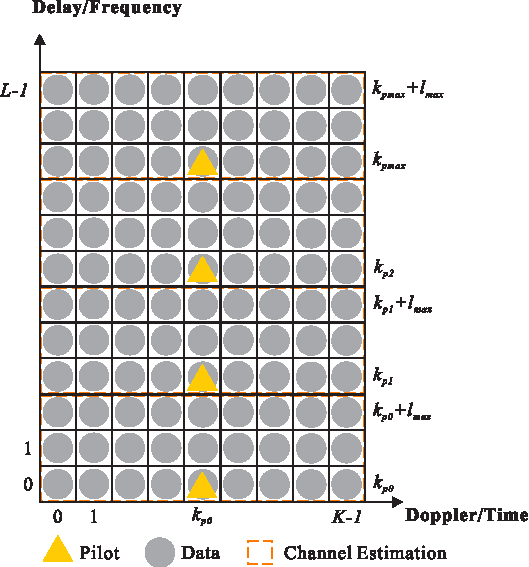
\includegraphics[width=\linewidth]{otfs_frame}
    \caption{OTFS frame structure}
    \label{fig:otfs_frame}
\end{figure}


We consider an OTFS system that transmits symbols $\bm{X_{D}}\in \mathbb{C}^{K\times L}$ over the delay-Doppler (DD) domain grids $\{(k\Delta\tau, l\Delta v)|k=0,...,K-1, l=0,...,L-1\}$, where $\Delta\tau$ and $\Delta v$ denote the delay and Doppler resolutions, where:
\begin{itemize}[label={--}] % 用横线代替默认的圆点
    \item $\Delta\tau=T/L$ is the delay resolution, with $T$ being the symbol duration of the OTFS system,
    \item $\Delta v=\Delta f/$ is the Doppler resolution, with $\Delta f=1/T$ denoting the subcarrier spacing.
\end{itemize}

The system bandwidth is $L\Delta f$, and the OTFS frame duration is $NT$. The transmitter first maps the symbols $x[k,l]$ to the time-frequency (TF) domain grids $\{(l\Delta f, kT)|\}$ via the inverse finite symplectic Fourier transform (ISFFT). The time-domain signal is synthesized using a conventional OFDM modulator with a transmit shaping pulse yet employs a single initial cyclic prefix spanning the full delay-Doppler spread duration, contrasting with conventional OFDM's per-symbol cyclic prefix insertion. The time-domain signal is transmitted over a time-varying wireless channel characterized by the delay-Doppler impulse response $h(\tau, v)$ as \cite{7925924},
\begin{equation}
h(\tau, v) = \sum_{i=1}^P h_i \delta (\tau - {\tau}_i) \delta (v - v_i) ,
\end{equation}
where $\delta(\cdot)$ denotes the Dirac delta function, $h_i \sim \mathcal{N}(0, \frac{1}{P})$ is the gain of the $i$-th propagation path, and $P$ represents the total number of paths. Each path is characterized by distinct delay and/or Doppler shifts, modeling the channel response between the receiver and either moving reflectors or the transmitting source. The delay and Doppler shifts are given as,
\begin{equation}
{\tau}_i = l_i \frac{T}{L}, v_i = k_i \frac{\Delta f}{K},
\end{equation}
respectively. Let the integers $l_i \in [0, l_{max}]$ and $k_i \in [-k_{max}, k_{max}]$ represent the delay and Doppler shift indices, respectively, where $l_{max}$ and $k_{max}$ denote the maximum delay index and maximum Doppler shift index across all propagation paths. Note that we restrict our consideration to integer-valued indices, as fractional delay and Doppler shifts can be equivalently represented through virtual integer taps in the delay-Doppler domain using the techniques described in \cite{6563167, 8377159, 8516353}.

At the receiver, the time-domain signal is first converted to the time-frequency (TF) domain through matched filtering and OFDM demodulation, then transformed to the delay-Doppler (DD) domain via inverse symplectic finite Fourier transform (ISFFT), yielding the received symbols $\bm{Y}_D\in \mathbb{C}^{K\times L}$. The DD domain input-output relationship can be formulated in vector form as \cite{10264119},
\begin{equation}
\bm{y} = \bm{Hx} + \bm{\tilde{z}},
\label{eq:sys-DD}
\end{equation}
where $\bm{x} = vec(\bm X_D^T)$, $\bm y = vec(\bm Y_D^T)$, and $\tilde{z} \sim \mathcal{CN}(0, \sigma_z^2)$ is an independent and identically distributed (i.i.d.) Gaussian noise \cite{8516353, 10264119, 7925924}.

%% todo
% 解释 H 在两种Pulse的值


\section{Joint Parallel Interference Cancellation Network}
% todo
% Fig.\ref{}

In this section, we propose a novel JPICNet framework that enhance the joint PIC scheme with graph neural network. Fig.\ref{} illustrates the process of the proposed framework. The proposed framework consists of channel parameters estimation (CPE), the GNN-aided symbol detection (GSD) and the GNN-aided channel estimation (GCHE) modules. CPE runs only once to generate initial input for GSD, while GSD and GCHE iteratively exchange outputs in a feedback loop.

\subsection{Channel Parameters Estimation}
% todo
% Estimation area
Estimation area $k \in [0, K-1], l \in [0, lmax]$

Based on the transmission arrangement, we can express the received signal in the channel estimation area as,
\begin{equation}
\begin{split}
y[k, l] = &h[k - k_p, l-{l_p}_0]x_p \\
& + \sum_i^P h_i \beta[k, l, k_i, l_i] x_d[[k-k_i]_K, [l-l_i]_L]\\
& + \tilde{z}[k, l].
\end{split}
\label{eq:JPICNet-CPE-rxSigCHE}
\end{equation}
%The parameter $\beta[k, l, k_i, l_i]$ corresponds to OTFS with ideal waveform is given as,
%\begin{equation}
%    \beta[k, l, k_i, l_i] = e^{-j2\pi  \frac{k_il_i}{KL}}, 
%\end{equation}
%while $\beta[k, l, k_i, l_i]$ applies to OTFS with rectangular waveform is given as,
%
%\begin{equation}
%\beta[k, l, k_i, l_i] = 
%\begin{cases}
%   	e^{j2\pi  \frac{k_i(l-l_i)}{KL}} & l_i \leq l < L, \\
%   	e^{-2j\pi \left( \frac{[k-k_i]_K}{K}\right)}e^{j2\pi \frac{k_i(l-l_i)}{KL}} & 0 	\leq l < l_i. \\
%\end{cases}
%\end{equation}
The parameter $\beta[k, l, k_i, l_i]$ has distinct forms for different OTFS waveforms:
\begin{enumerate}
	\renewcommand{\labelenumi}{\roman{enumi})} % 小写罗马数字 + 右括号
    \item \textit{Ideal waveform}:
    \begin{equation}
        \beta_{\text{ideal}}[k, l, k_i, l_i] = e^{-j2\pi \frac{k_i l_i}{KL}},
    \end{equation}
    \item \textit{Rectangular waveform}:
    \begin{equation}
    \begin{split}
        & \beta_{\text{rect}}[k, l, k_i, l_i] =  \\
        & \hspace{1em}\begin{cases}
            e^{j2\pi \frac{k_i(l-l_i)}{KL}}, & l_i \leq l < L, \\
            e^{-j2\pi \left(\frac{[k-k_i]_K}{K}\right)} e^{j2\pi \frac{k_i(l-l_i)}{KL}}, & 0 \leq l < l_i.
        \end{cases}
    \end{split}
    \end{equation}
\end{enumerate}
From \eqref{eq:JPICNet-CPE-rxSigCHE}, the second term arises from the interference between pilot and data symbols. For simplicity, this cross-interference can be modeled as an additive noise term in subsequent analysis, i.e.,
\begin{equation}
\mathcal{I}[k, l] = \sum_i^P h_i \beta[k, l, k_i, l_i] x_d[[k+k_i]_K, [l+l_i]_L].
\end{equation}
The interference term $\mathcal{I}[k, l]$ is zero-mean ($\mathbb{E}[\mathcal{I}\{[k, l]\}=0$) with its variance given by,
\begin{equation}
\text{Var}(\mathcal{I}[k, l]) = \sigma_d^2.
\end{equation}
\begin{proof}
The proof is given in Appendix~\ref{app:cpe-inter-mu-var}.
\end{proof}

Based on the received signal model in \eqref{eq:JPICNet-CPE-rxSigCHE}, we propose a threshold-based channel estimation algorithm as follows. For each delay-Doppler bin $[k,l]$, if the received energy $|y[k, l]|^2$ falls below a predefined threshold $\mathcal{T}$, we declare an empty bin (no path present). Otherwise, we obtain an initial channel estimate as,
%\begin{equation}
%\hat{h}[k - k_p, l-{l_p}_0]= [|x_p|^2 + P(\sigma_z^2+\sigma_d^2)]^{-1}x_p^*y[k,l]
%\end{equation}
\begin{equation}
\hat{h}[k - k_p, l-{l_p}_0]= y[k,l]/x_p.
\end{equation}
Therefore, the threshold provides a mask vector to indicate whether there is a path locating at the delay vector $\bm k_m$ and Doppler vector $\bm l_m$, i.e,
\begin{subequations}
\begin{align}
\bm h_m = & [h_{m0}, \cdots, h_{mi}, \cdots, h_{mP_{max}}], \label{eq:CPE-hm} \\
\bm k_m = & [-k_{max}, \cdots, 0, \cdots, k_{max}, \cdots, k_{mi} \\
& \cdots, -k_{max}, \cdots, 0, \cdots, k_{max}],
\label{eq:CPE-km} \\
\bm l_m = & [0, 1, \cdots, l_{max}, \cdots, l_{mi}, \cdots, 0, 1, \cdots, l_{max}]. \label{eq:CPE-lm}
\end{align}
\end{subequations}
where $h_{mi} = 1 $ denotes a path at $( k_{mi}, l_{mi})$ and 0 otherwise, and $P_{max} = (l_{max}+1)(2k_{max}+1))$.


%% todo
% \hat{H}
% V_\hat{H}

\subsection{GNN-aided Symbol Detection}
At each iteration $t$, the symbol vector $\bm{x}$ defined in \eqref{eq:sys-DD} is treated as a random vector, with its statistical parameters estimated from the observation $\bm{y}$. based on the same equation. The conditional Gaussian probability distribution
function (PDF) is subsequently derived as,
\begin{equation}
p^{(t)}=(\bm{x}|\bm{y}) = \mathcal{N}(\bm{x}, \bm{\mu}_{\bm{x}}^{(t)}; \Sigma_{\bm{x}}^{(t)}),
\end{equation}
where
\begin{subequations}
\begin{align}
\bm{\mu}_{\bm{x}}^{(t)} &= (\bm I\odot\hat{\bm H}^{(t)^H} \hat{\bm H}^{(t)})^{-1}\hat{\bm H}^{(t)^H}y, \label{eq:GSD-mean} \\
\Sigma_{\bm{x}}^{(t)} &= (\sigma_z^2 + \sigma_x^2 D_{\Delta \hat{\bm H}})(\bm I\odot\hat{\bm H}^{(t)^H} \hat{\bm H}^{(t)})^{-1}. \label{eq:GSD-cov} \\
\end{align}
\end{subequations}
where
\begin{equation}
D_{\Delta \hat{\bm H}} = diag(\sum_{i=0}^{KL-1}\bm \Sigma_{\hat{\bm H}}[:, i]),
\end{equation}
$\Sigma_{\hat{\bm H}}$ denotes the variance matrix of $\hat{\bm H}$, and $\sum_{i=0}^{KL-1}\bm \Sigma_{\hat{\bm H}}[:, i]$ means we sum all columns of $\Sigma_{\hat{\bm H}}$ together to build a column vector.

\begin{proof}
The proof is given in Appendix~\ref{app:GSD}.
\end{proof}

% todo
% X

\subsection{GNN-aided Channel Estimation}
Rewriting \eqref{eq:sys-DD} for channel estimation, we have
\begin{equation}
\bm y = \bm\Phi \bm h + \bm{\tilde{z}},
\label{eq:GCHE-sys}
\end{equation}
where $\bm h$ is the path gain in the time domain,  
\[
\begin{split}
& \bm\Phi = \\
& \begin{bmatrix}
    \Phi_{k_{m0}, l_{m0}}(1, 1) & \cdots & \Phi_{k_{mP_{max}}, l_{k_{mP_{max}}}}(KL, P_{max}) \\ 
	\vdots & \ddots  & \vdots \\  
    \Phi_{k_{m0}, l_{m0}}(KL, 1) & \cdots & \Phi_{k_{mP_{max}}, l_{k_{mP_{max}}}}(KL, P_{max}) \\
\end{bmatrix},
\end{split}
\]
where $(kL+l, i)$th entry of $\Phi \in \mathcal{C}^{(KL-1)\times P_{max}}$ is \cite{9785832},
\begin{dmath}
\Phi_{k_{mi}, l_{mi}}(kL+l, i) = X([k-k_{mi}]_K, [l-l_{mi}]_L)\beta[k, l, k_{mi}, l_{mi}].
\end{dmath}
However, we use the estimation of $\Phi$



Inspired by \cite{945004, 5493831}, we implement a linear minimum-mean-squared
error (MMSE) channel estimation , i.e.,
\begin{subequations}
\begin{align}
\hat{\bm h}^{(t)} = & \hspace{0.3em} \bm R_{\bm h}\bm\Phi^{(t)^H}(\bm \Phi^{(t)}R_{\bm h}\bm\Phi^{(t)^H}\bm + \notag \\
& \hspace{0.3em} \frac{1}{P} diag(\bm h_m) D_{\Delta \Phi^{(t)}} +\sigma_z^2\bm I)^{-1}\bm y, \label{eq:GCHE-mean} \\
\text{Var}(\hat{\bm h}^{(t)}) = & \hspace{0.3em} \bm R_{\bm h} - \bm R_{\bm h}\Phi^{(t)^H} (\bm \Phi^{(t)} R_{\bm h} \bm\Phi^{(t)^{H}}\bm + \notag\\
\hspace{0.3em}& \frac{1}{P} diag(\bm h_m) D_{\Delta \Phi^{(t)}} +\sigma_z^2\bm I))^{-1} \Phi^{(t)}\bm R_{\bm h} \label{eq:GCHE-var}, \\
\end{align}
\end{subequations}
where $\bm\Phi^{(t)}$ is the estimation of $\bm\Phi$ in $t$-th iteration, and,
\begin{equation}
D_{\Delta \Phi^{(t)}} = diag(\sum_{i=0}^{KL-1}\bm \Sigma_{\Delta \Phi^{(t)}}[:, i]).
\end{equation}
$\Sigma_{\Delta\Phi^{(t)}}$ denotes the variance matrix of $\Phi^{(t)}$, and $\sum_{i=0}^{KL-1}\bm \Sigma_{\Delta \Phi^{(t)}}[:, i]$ means we sum all columns of $\Sigma_{\Delta\Phi^{(t)}}$ together to build a column vector.

\begin{proof}
The proof is given in Appendix~\ref{app:GCHE}.
\end{proof}


%%%%%%%%%%%%%%%%%%%%%%%%%%%%%%%%%%%%%%%%%%%%%%%%%%%%%%%%%%%%%%%%%%%%
% appendix
\appendices
\section{CPE Cross-Interference} \label{app:cpe-inter-mu-var}
\begin{multline}
\mathbb{E}\{\mathcal{I}[k, l]\} = \sum_{i=1}^P \underbrace{\mathbb{E}\{h_i\}}_{0} \beta[k, l, k_i, l_i] \\
\underbrace{\mathbb{E}\{x_d[[k+k_i]_K, [l+l_i]_L]\}}_{0} = 0
\end{multline}

\begin{equation}
\text{Var}(\mathcal{I}[k, l]) = \mathbb{E}\left\{ |\mathcal{I}[k, l]|^2 \right\},
\end{equation}
where
\begin{multline}
|\mathcal{I}[k, l]|^2 = \sum_{i=1}^P |h_i|^2 |\beta[k, l, k_i, l_i]|^2
|x_d[[k+k_i]_K, [l+l_i]_L]|^2 \\
+ \sum_{i \neq j} h_ih_j^*\beta[k, l, k_i, l_i]\beta[k, l, k_j, l_j]^*\cdot \\
x_d[[k+k_i]_K, [l+l_i]_L]x_d[[k+k_j]_K, [l+l_j]_L]^*
\label{app:cpe-inter-mu-var:inter-sqr}
\end{multline}
The expectation of the second term in \eqref{app:cpe-inter-mu-var:inter-sqr} vanishes because $\mathbb{E}\{h_i h_j^*\} = 0$, i.e.,
\begin{equation}
\begin{split}
\text{Var}(\mathcal{I}[k, l]) =& \sum_{i=1}^P \underbrace{|h_i|^2}_{1/P} \cdot \underbrace{|\beta[k, l, k_i, l_i]|^2}_{1} \cdot \\
&\underbrace{|x_d[[k+k_i]_K, [l+l_i]_L]|^2}_{\sigma_d^2}\\
=& \sum_{i=1}^P 1/P\cdot\sigma_d^2 = \sigma_d^2
\end{split}
\end{equation}


\section{GSD Variance} \label{app:GSD}
For simplification, we denote $\hat{\bm H}^{(t)}$ as $ \hat{\bm H}$ and the power of $\bm x$ as $\sigma_x^2$. Therefore, the estimated symbol is
\begin{equation}
\begin{split}
\bm {\mu}_{\bm x} = \hspace{0.3em}& (\bm I\odot\hat{\bm H}^H \hat{\bm H})^{-1}\hat{\bm H}^H\bm y, \\
= \hspace{0.3em}& (\bm I\odot\hat{\bm H}^H \hat{\bm H})^{-1}\hat{\bm H}^H(\bm H \bm x + \tilde{\bm z}), \\
= \hspace{0.3em}& \underbrace{(\bm I\odot\hat{\bm H}^H \hat{\bm H})^{-1}\hat{\bm H}^H}_{{\bm W}_{GSD}} \times \\
& (\hat{\bm H} \bm x + \bm H \bm x - \hat{\bm H} \bm x + \tilde{\bm z}), \\
= \hspace{0.3em} & {\bm W}_{GSD} (\hat{\bm H} \bm x + \Delta\hat{\bm H} \bm x + \tilde{\bm z}), \\
= \hspace{0.3em} & {\bm W}_{GSD}\hat{\bm H} \bm x + {\bm W}_{GSD}\Delta H\bm x +  {\bm W}_{GSD}\tilde{\bm z}.
\end{split}
\end{equation}
The estimation error is
\begin{equation}
\begin{split}
\bm e &= \bm {\mu}_{\bm x} - \bm x, \\
&= ({\bm W}_{GSD}\hat{\bm H} - \bm I) \bm x + {\bm W}_{GSD}\Delta H\bm x + {\bm W}_{GSD}\tilde{\bm z}.
\end{split}
\end{equation}
Please note $\hat{\bm H}$ is the estimation of $\bm H$, i.e., $\mathbb{E}\{\Delta\hat{\bm H} \}=0$ and $\mathbb{E}\{ \tilde{\bm z}\}=0$. Therefore, the corvariance of $\bm {\mu}_{\bm x}$ is,
\begin{equation}
\begin{split}
\text{Cov}(\bm {\mu}_{\bm x}) = \hspace{0.3em} & \mathbb{E}\{\bm e \bm e^H\}, \\
=\hspace{0.3em} & \mathbb{E}\{({\bm W}_{GSD}\hat{H} - \bm I)\bm x \bm x^H ({\bm W}_{GSD}\hat{H} - \bm I)^H\} \\
& + \mathbb{E}\{ {\bm W}_{GSD}\Delta \hat{\bm H} \bm x \bm x^H \Delta \hat{\bm H}^H{\bm W}_{GSD}^H\} \\ 
& + \mathbb{E}\{ {\bm W}_{GSD}\tilde{\bm z}\tilde{\bm z}^H{\bm W}_{GSD}^H \}, \\
=\hspace{0.3em} & \sigma_x^2\mathbb{E}\{({\bm W}_{GSD}\hat{H} - \bm I)({\bm W}_{GSD}\hat{H} - \bm I)^H\} \\
& + \sigma_x^2\mathbb{E}\{{\bm W}_{GSD} \Delta \hat{\bm H} \Delta \hat{\bm H}^H{\bm W}_{GSD}^H\} \\ 
& + \sigma_z^2\mathbb{E}\{ {\bm W}_{GSD}{\bm W}_{GSD}^H \}. \\
\end{split}
\label{app:GSD-var:cov-1}
\end{equation}
Since the estimated channel coefficients are assumed to be mutually independent, the first term in \eqref{app:GSD-var:cov-1} can thus be simplified as,
\begin{equation}
\begin{split}
& \sigma_x^2\mathbb{E}\{({\bm W}_{GSD}\hat{H} - \bm I)({\bm W}_{GSD}\hat{H} - \bm I)^H\}\\
=\hspace{0.3em} & \sigma_x^2\mathbb{E}\{{\bm W}_{GSD}\hat{\bm H}\hat{\bm H}^H{\bm W}_{GSD}^H - \bm I\}, \\
=\hspace{0.3em} & \sigma_x^2\mathbb{E}\{ (\bm I\odot\hat{\bm H}^H \hat{\bm H})^{-1}\hat{\bm H}^H \hat{\bm H}\hat{\bm H}^H \hat{\bm H} (\bm I\odot\hat{\bm H}^H \hat{\bm H})^{-1} \\
& - \bm I\}, \\
=\hspace{0.3em} & \sigma_x^2\mathbb{E}\{ \bm I - \bm I\} = \bm 0.
\end{split}
\end{equation}
Similarly, the last term in \eqref{app:GSD-var:cov-1} can be simplified as,
\begin{equation}
\begin{split}
 \hspace{0.3em}&\sigma_z^2\mathbb{E}\{ {\bm W}_{GSD}{\bm W}_{GSD}^H \} \\
=\hspace{0.3em} & \sigma_z^2\mathbb{E}\{(\bm I\odot\hat{\bm H}^H \hat{\bm H})^{-1}\hat{\bm H}^H \hat{\bm H} (\bm I\odot\hat{\bm H}^H \hat{\bm H})^{-1} \}, \\
=\hspace{0.3em} & \sigma_z^2(\bm I\odot \hat{\bm H}^H \hat{\bm H})^{-1}.
\end{split}
\end{equation}
Therefore, \eqref{app:GSD-var:cov-1} can be written as,
\begin{equation}
\begin{split}
\text{Cov}(\bm {\mu}_{\bm x}) = \hspace{0.3em}& \sigma_x^2\mathbb{E}\{\bm W_{GSD} \bm D_{\Delta \hat{\bm H}}{\bm W}_{GSD}^H\} \\
& + \sigma_z^2(\bm I\odot\hat{\bm H}^H \hat{\bm H})^{-1},
\end{split}
\end{equation}
The variance is the diagonal of $Cov(\bm {\mu}_{\bm x})$, i.e.,
\begin{equation}
\begin{split}
\text{Var}({{\mu}_{\bm x}}_i) = \hspace{0.3em}  & \sigma_z^2 \sum_{j=0}^{KL-1} |\hat{H}[j, i]|^{-2} + \\ 
& \sigma_x^2 \sum_{j=0}^{KL-1} |\hat{H}[j, i]|^{-2} \sum_{j'=0}^{KL-1} \sigma^2_{\hat{H}}[i, j'],
\end{split}
\end{equation}
where $\sigma^2_{\hat{H}}[j, i']$ is the $(j, i')$th entry of $\Sigma_{\hat{\bm H}}$.

\section{GCHE} \label{app:GCHE}
In $t$-th iteration, \eqref{eq:GCHE-sys} can be written as,
\begin{equation}
\begin{split}
\bm y &= (\bm\Phi^{(t)} + \bm\Phi - \bm\Phi^{(t)})\bm h + \tilde{\bm z}, \\
&= \bm\Phi^{(t)}\bm h + \Delta\bm\Phi^{(t)}\bm h + \tilde{\bm z}, \\ 
&= \bm\Phi^{(t)}\bm h + \tilde{\bm z}^{(t)},
\end{split}
\label{eq:GCHE-sys-est-1} 
\end{equation}
where $\mathbb{E}\{\Delta\bm\Phi^{(t)}\}=0$.
The mean of $\tilde{\bm z}^{(t)}$ is,
\begin{equation}
\begin{split}
\mathbb{E}\{\tilde{\bm z}^{(t)}\} &= \mathbb{E}\{ \Delta\bm\Phi^{(t)}\bm h \} + \mathbb{E}\{\tilde{\bm z} \}, \\
& = \Delta\bm\Phi^{(t)} \mathbb{E}\{ \bm h \} + \mathbb{E}\{\tilde{\bm z} \}, \\
&= \bm 0.
\end{split}
\end{equation}
The covariance of $\tilde{\bm z}^{(t)}$ is,
\begin{equation}
\begin{split}
\text{Cov}(\tilde{\bm z}^{(t)}) &= \bm R_{\tilde{\bm z}^{(t)}}, \\
&= \bm R_{\Delta\bm\Phi^{(t)}\bm h} + \bm R_{\tilde{\bm z}}, \\
&= \mathbb{E}\{\Delta\bm\Phi^{(t)}\bm h \bm h^H \Delta\bm\Phi^{(t)^H} \} + \sigma_z^2\bm I, \\
&= \frac{1}{P} \mathbb{E}\{\Delta\bm\Phi^{(t)} diag(\bm h_m) \Delta\bm\Phi^{(t)^H} \}, \\
&= \frac{1}{P} diag(\bm h_m) D_{\Delta \Phi^{(t)}}.
\end{split}
\end{equation}
Therefore, the linear MMSE estimation is,
\begin{dmath}
\hat{\bm h}^{(t)} = \bm R_{\bm h}\bm\Phi^{(t)^H}(\bm \Phi^{(t)}\bm R_{\bm h}\bm\Phi^{(t)^H} + \frac{1}{P} diag(\bm h_m) D_{\Delta \Phi^{(t)}} +\sigma_z^2\bm I)^{-1}\bm y.
\end{dmath}
The covariance of the estimation error is,
\begin{equation}
\begin{split}
\text{Var}(\bm e) = \hspace{0.3em}& \mathbb{E}\{ (\bm h - \bm\hat{h}^{(t)})(\bm h - \bm\hat{h}^{(t)})^H \}, \\
=\hspace{0.3em}& \mathbb{E}\{\bm h \bm h^H\} - \mathbb{E}\{\hat{\bm h}\hat{\bm h}^H\}, \\
=\hspace{0.3em}& \bm R_{\bm h} - \bm R_{\bm h}\Phi^{(t)^H}\bm R_{\bm y}^{-1}R_{\bm y}R_{\bm y}^{-1}\Phi^{(t)}\bm R_{\bm h}, \\
=\hspace{0.3em}& \bm R_{\bm h} - \bm R_{\bm h}\Phi^{(t)^H}R_{\bm y}^{-1}\Phi^{(t)}\bm R_{\bm h}, \\
=\hspace{0.3em}& \bm R_{\bm h} - \bm R_{\bm h}\Phi^{(t)^H} (\bm \Phi^{(t)} R_{\bm h} \bm\Phi^{(t)^{H}}\bm + \\
\hspace{0.3em}& \frac{1}{P} diag(\bm h_m) D_{\Delta \Phi^{(t)}} +\sigma_z^2\bm I))^{-1} \Phi^{(t)}\bm R_{\bm h}, \\
\end{split}
\end{equation}


%\underbrace{
%Therefore, the estimation error is,
%\begin{equation}
%\begin{split}
%\bm e &= \bm y - \bm \phi \hat{h} \\
%&= \bm y - \phi\bm R_{\bm h}(\bm \Phi^{(t)^H}\bm\Phi^{(t)}\bm diag(\bm h) + \sigma_z^2\bm I)^{-1}\bm\Phi^H\bm y
%\end{split}
%\end{equation}


{\renewcommand{\baselinestretch}{1.1}
\begin{footnotesize}
\bibliographystyle{IEEEtran}
\bibliography{myBib}
\end{footnotesize}}

\end{document}
